\documentclass{letask}
\usepackage{wrapfig}
\usepackage{ctable}
\begin{document}
\begin{titlepage}
\center % Center everything on the page
 
%----------------------------------------------------------------------------------------
%	HEADING SECTIONS
%----------------------------------------------------------------------------------------

\textsc{\LARGE Московский\\[-0.2cm]Физико-Технический Институт\\[0.1cm]\large (государственный университет)}\\[1.5cm] % Name of your university/college
\textsc{\Large Кафедра общей физики}\\[0.1cm] % Major heading such as course name
\textsc{\large Лабораторная работа \textnumero  4.7.2}\\[0.5cm] % Minor heading such as course title

%----------------------------------------------------------------------------------------
%	TITLE SECTION
%----------------------------------------------------------------------------------------

\HRule
\\[0.6cm]
{ \huge \bfseries Эффект Поккельса}
\\[0.4cm] % Title of your document
\HRule
\\[1.5cm]


 
%----------------------------------------------------------------------------------------
%	AUTHOR SECTION
%----------------------------------------------------------------------------------------

\begin{minipage}{0.4\textwidth}
	\begin{flushleft} \large
		\textsf{Студент}
		
		Алексей \textsc{Домрачев} \\[-0.15cm]
		615 группа
	\end{flushleft}
\end{minipage}
~
\begin{minipage}{0.4\textwidth}
	\begin{flushright} \large
		\textsf{Преподаватель}
		
		Андрей Александрович\\[-0.15cm]
		\textsc{Заболотных} % Supervisor's Name
	\end{flushright}
\end{minipage}

\begin{bottompar}
	\begin{center}
		
\includegraphics[width = 80 mm]{logo.jpg}
	\end{center}
	{\large \today}

\end{bottompar}
\vfill % Fill the rest of the page with whitespace

\end{titlepage}

\paragraph{Цель работы:} исследовать интерференцию рассеянного света, прошедшего кристалл; наблюдать изменение характера поляризации света при наложении на кристалл электрического поля.
\paragraph{В работе используются:} гелий-неоновый лазер, поляризатор, кристалл ниобата лития, матовая пластинка, экран, источник высоковольтного переменного и постоянного напряжения, фотодиод, осциллограф, линейка.
\paragraph{Теоретическая справка.} Эффектом Поккельса называется изменение показателя преломления света в кристалле под действием электрического поля, причём это изменение пропорционально напряжённости электрического поля.

Во время обработки результатов мы воспользуемся формулой, выражающей зависимость квадрата радиуса m-ого темного кольца на коноскопической картине от $ m $:
\begin{equation}
	r_m^2 = \dfrac{\lambda}{l}\dfrac{\left( n_0L\right)^2}{(n_0-n_e)}m
\end{equation}

%тут будут формулы отвечаю

\paragraph{Выполнение работы.}
Соберем оптическую схему согласно рис 1. Проведем настройку
\begin{wrapfigure}[11]{l}{100mm}
	\label{scheme1}
	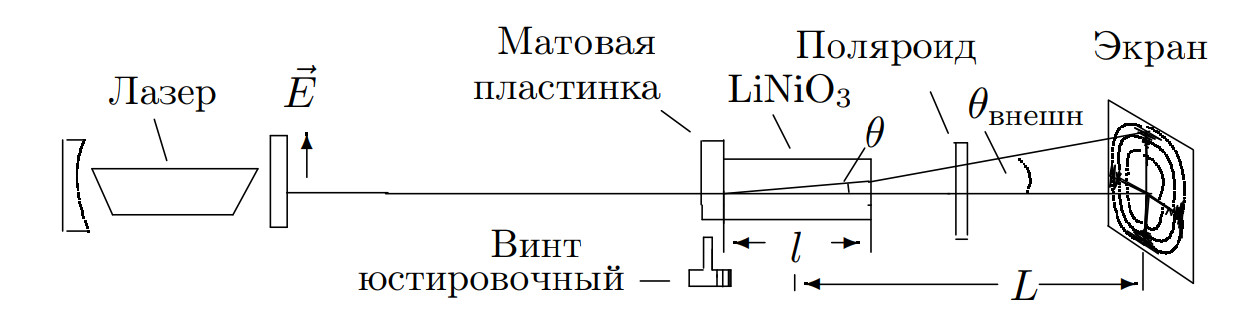
\includegraphics[width=100mm]{scheme1}
	\caption{Схема для наблюдения коноскопической картины.}
\end{wrapfigure}
 поляроида, с помощью света, который отражается от стола, на который направлена лампа, добьемся минимума освещенности, угол на лимбе при этом равен 21$ ^\circ $. Включив лазер мы получили коноскопическую картину(рис 2). Измерим расстояние от кристалла до экрана $ L = 85 \pm 0.2$ см. Также измерим радиусы темных колец и занесем их в таблицу \ref{table1}

\begin{minipage}{70mm}
 \begin{figure}[H]
 	\includegraphics[width=60mm]{inter_1}
 \end{figure}
\end{minipage}
~
\begin{minipage}{95mm}
	\begin{table}[H]
		\centering
		\caption{Радиусы интерференционных колец}
		\label{table1}
		\begin{tabular}{|c|c|c|c|c|c|c|}
			$m$ & 1 & 2 & 3 & 4 & 5 & 6 \\ \midrule
			$r$, см & 3.0 & 4.4 & 5.4 & 6.3 & 7.0 & 7.7 \\ \midrule
			$r^2$, см$^2$ & 9.0 & 19.4 & 29.2 & 39.7 & 49.0 & 59.3 
		\end{tabular}
	\end{table}
Подадим на кристал постоянный ток. С увеличением напряжения на кристалле яркость пятна на экране увеличивается и достигает максимума при $ U_{\lambda/2} = 450 $ В, при $ U_\lambda = 2 U_{\lambda/2} = 900 $ В яркость снова становится минимальной.
\end{minipage}


Проделав то же самое для параллельных поляризаций лазера и поляроида, мы получили значения близкие к предыдущим: $ U_{\lambda/2} = 465 $ В, $ U_\lambda = 900 $ В.

Теперь подадим на кристал переменный ток и соберем схему согласно рис 2. По фигурам Лиссажу на экране осциллографа определим $ U_{\lambda/2} = 2 $ В для переменного тока.
\paragraph{Обработка результатов.} Изобразим график из данных в таблице 1 на рис. 3.

\begin{wrapfigure}[5]{r}{70mm}
	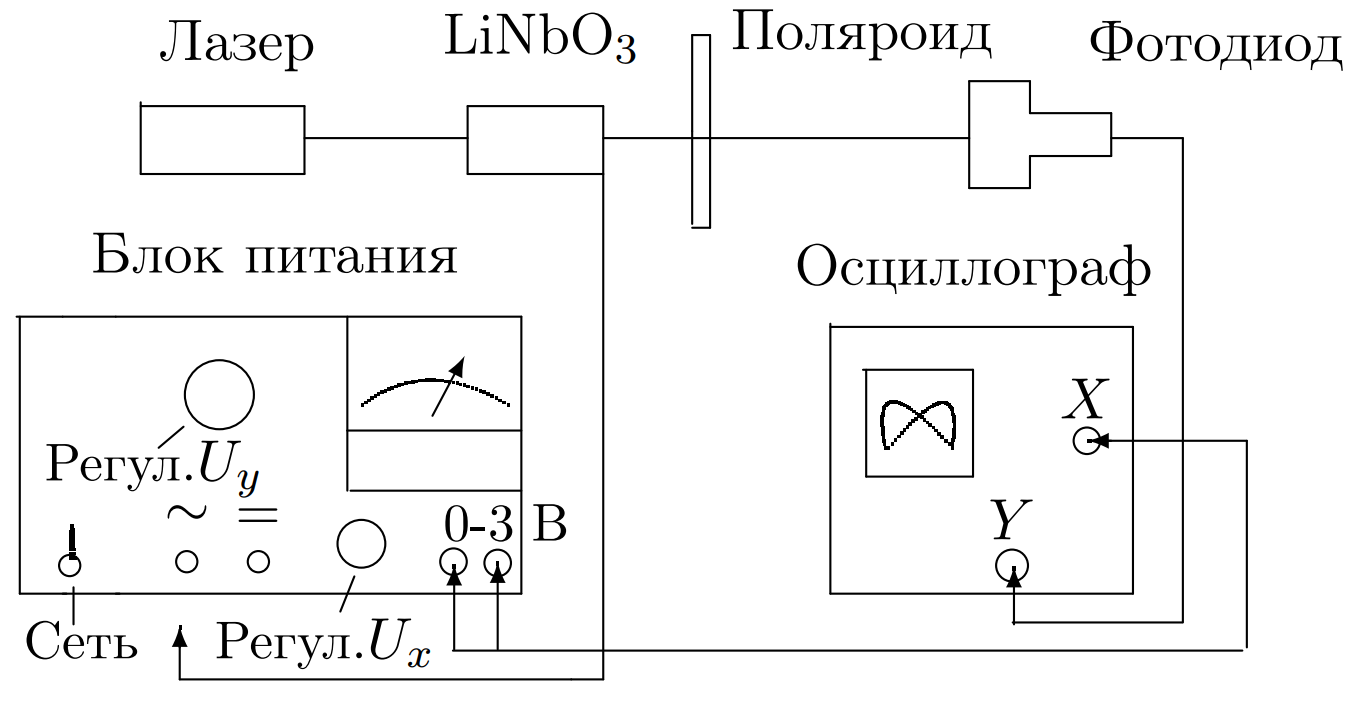
\includegraphics[width=70mm]{scheme2}
	\caption{Схема для изучения двойного лучепреломления в электрическом поле}
\end{wrapfigure}
С помощью МНК подсчитаем коэффициент наклона апроксимационной прямой. Получим, что ее коэффициент наклона $ b = 10.0 \pm 0.1 $ см$^2 = \\ = 10 \pm 0.1 \cdot 10^{-4}$ м$ ^2 $. Отсюда определим двулучепреломление $ (n_0-n_e) $ ниобата лития, из формулы (1)\\
$
	n_0-n_e=\frac{\lambda \left(  n_0 L \right)^2}{lb} = \frac{0.63\cdot(2.29\cdot0.85)^2}{0.026}\cdot10^{-3} = 9.2 \cdot 10^{-2}  
$

Рассчитаем погрешность этого измерения: \\$ \sigma_{n_0-n_e} = (n_0-n_e) \sqrt{4\cdot\varepsilon_L^2 + \varepsilon_b} = \\ =9.2\cdot 10^{-2} \cdot \sqrt{4\cdot (2\cdot 10^{-3})^2 + 0.01^2}  = 0.1 \cdot 10^{-2}  $

В итоге получаем : $	n_0 - n_e = 9.2 \pm 0.1 \cdot 10^{-2} $
\begin{figure}[H]
	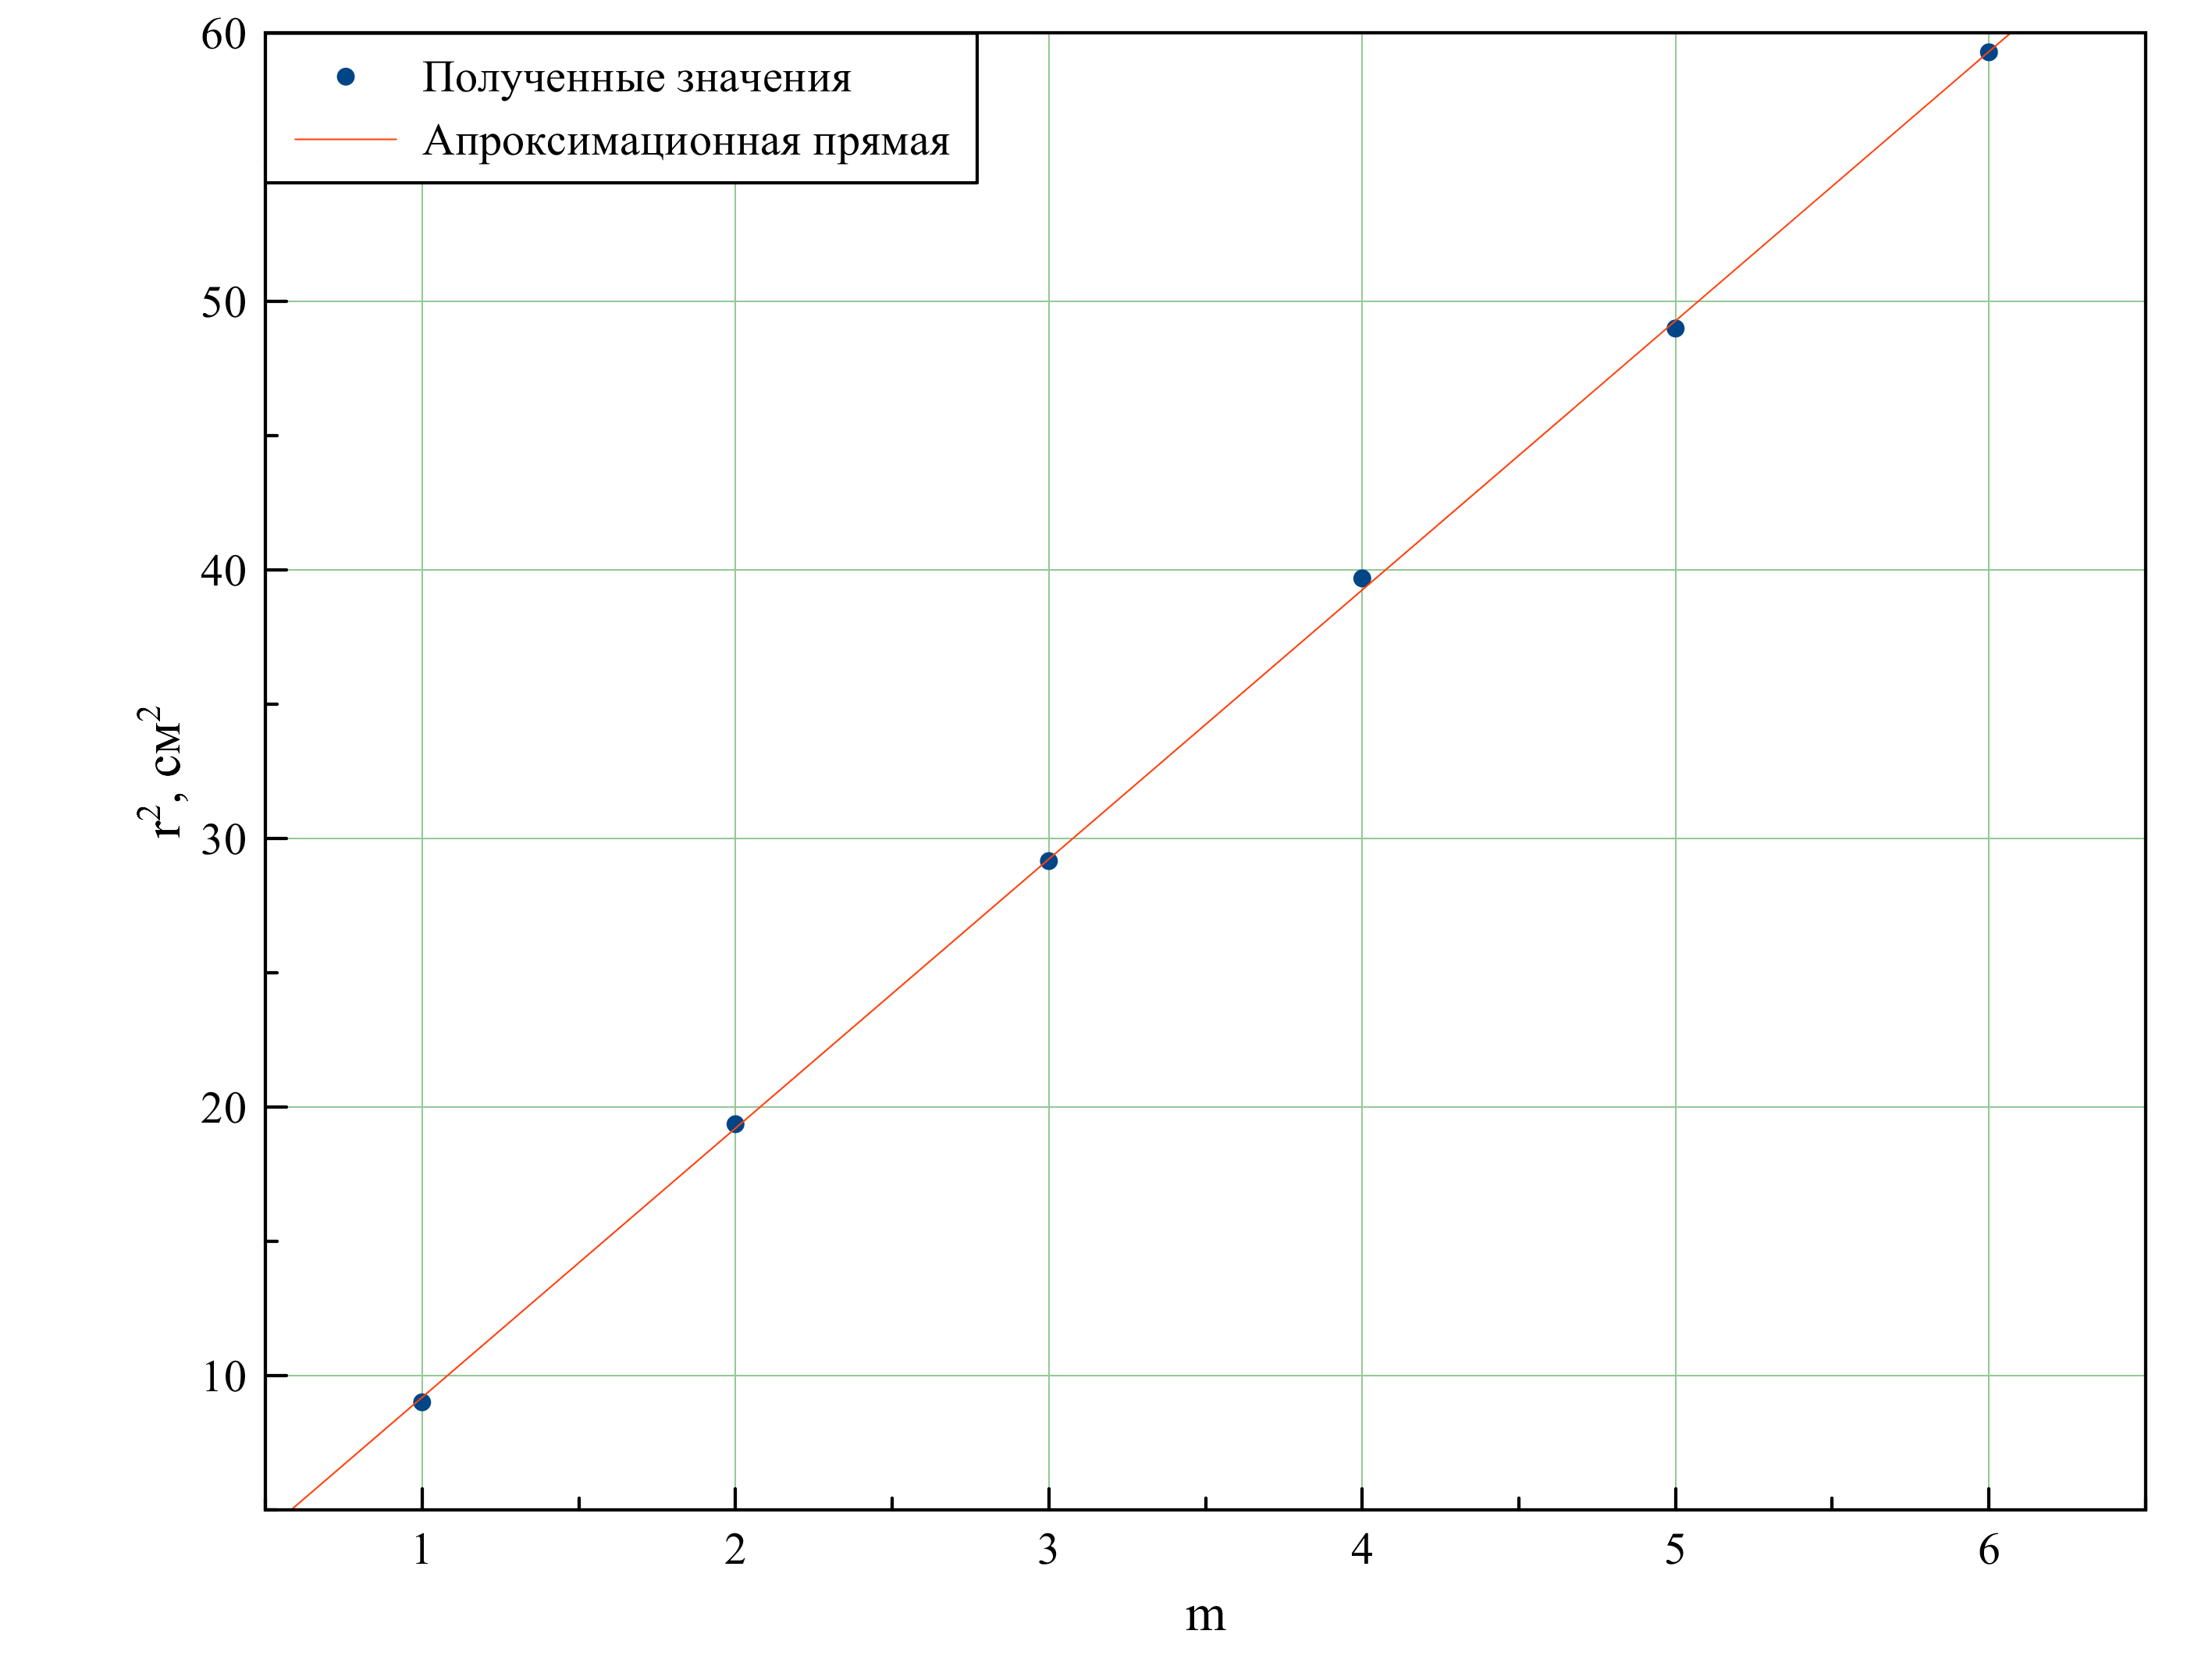
\includegraphics[width=130mm]{graph1}
	\caption{Зависимость квадрата радиуса от порядкового номера}
\end{figure}

Получим на экране осцилографа фигуры Лиссажу для напряжений $ U_{\lambda/2}, U_\lambda, U_{3\lambda/2} $ и сфотографируем их. 

\begin{figure}[H]
	\begin{minipage}[h]{0.32\linewidth}
		\center{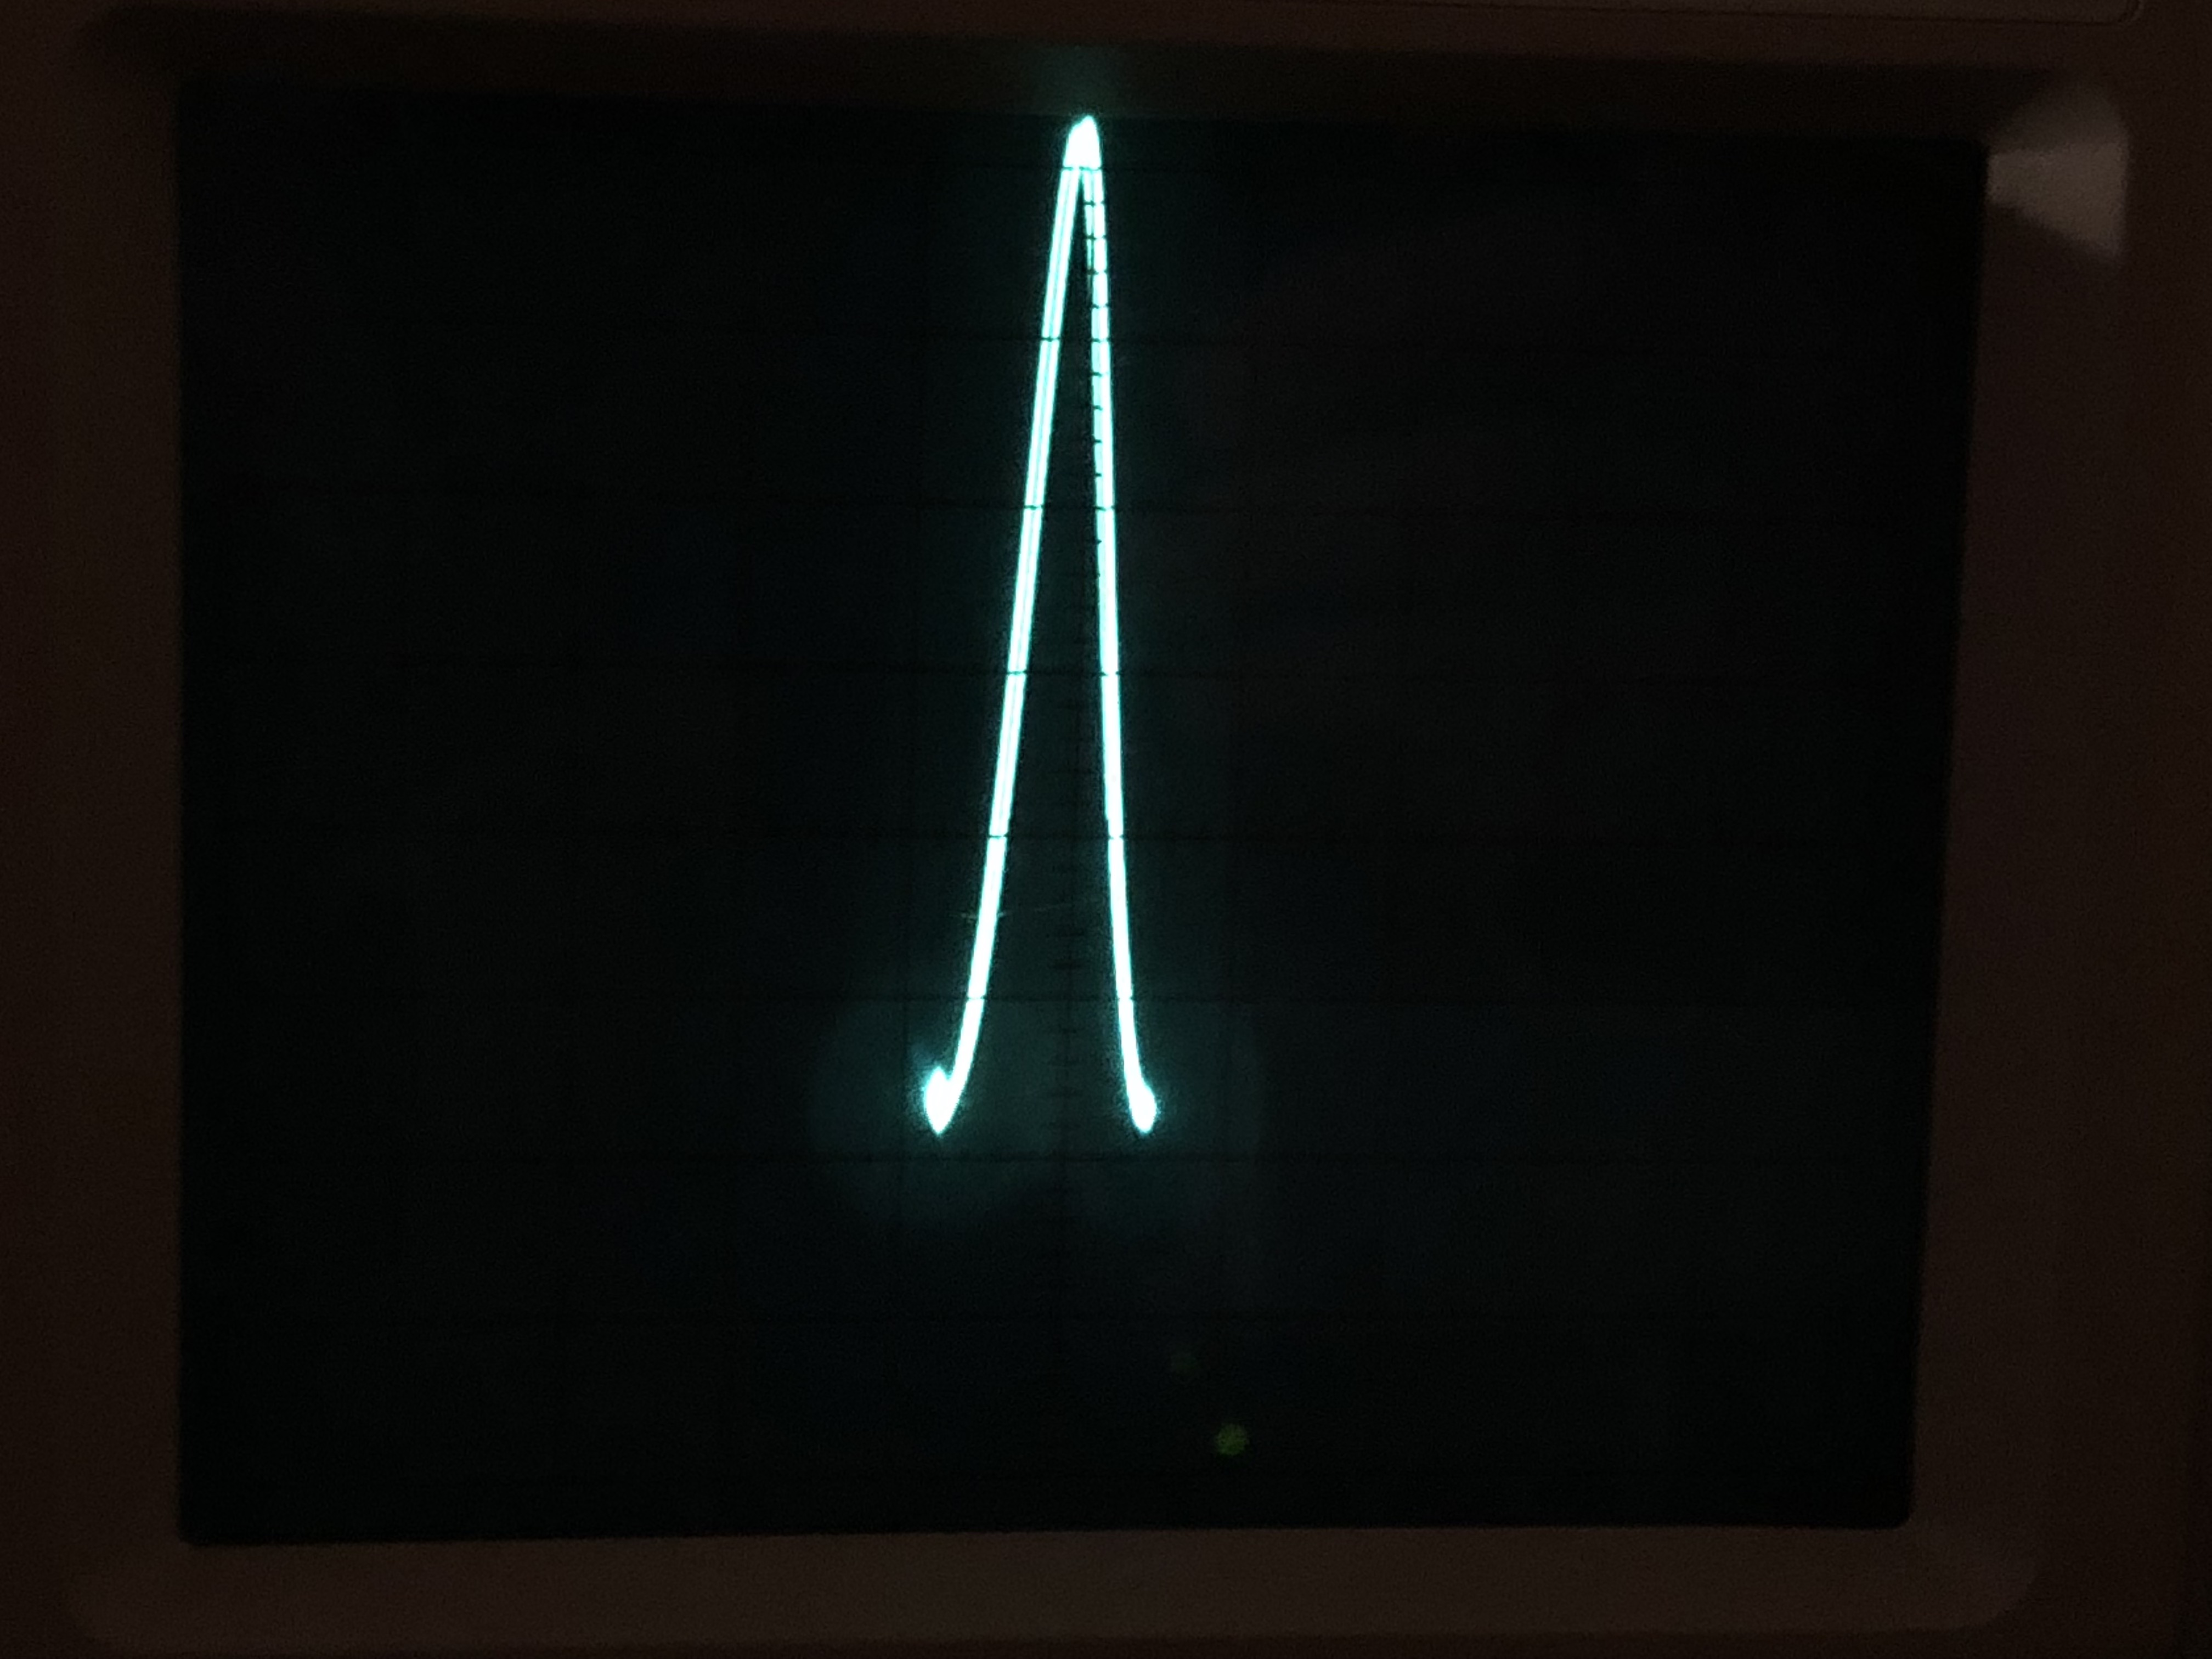
\includegraphics[width=0.7\linewidth]{lis1} \\ $  U_{\lambda/2} $}
	\end{minipage}
	\hfill
	\begin{minipage}[h]{0.32\linewidth}
		\center{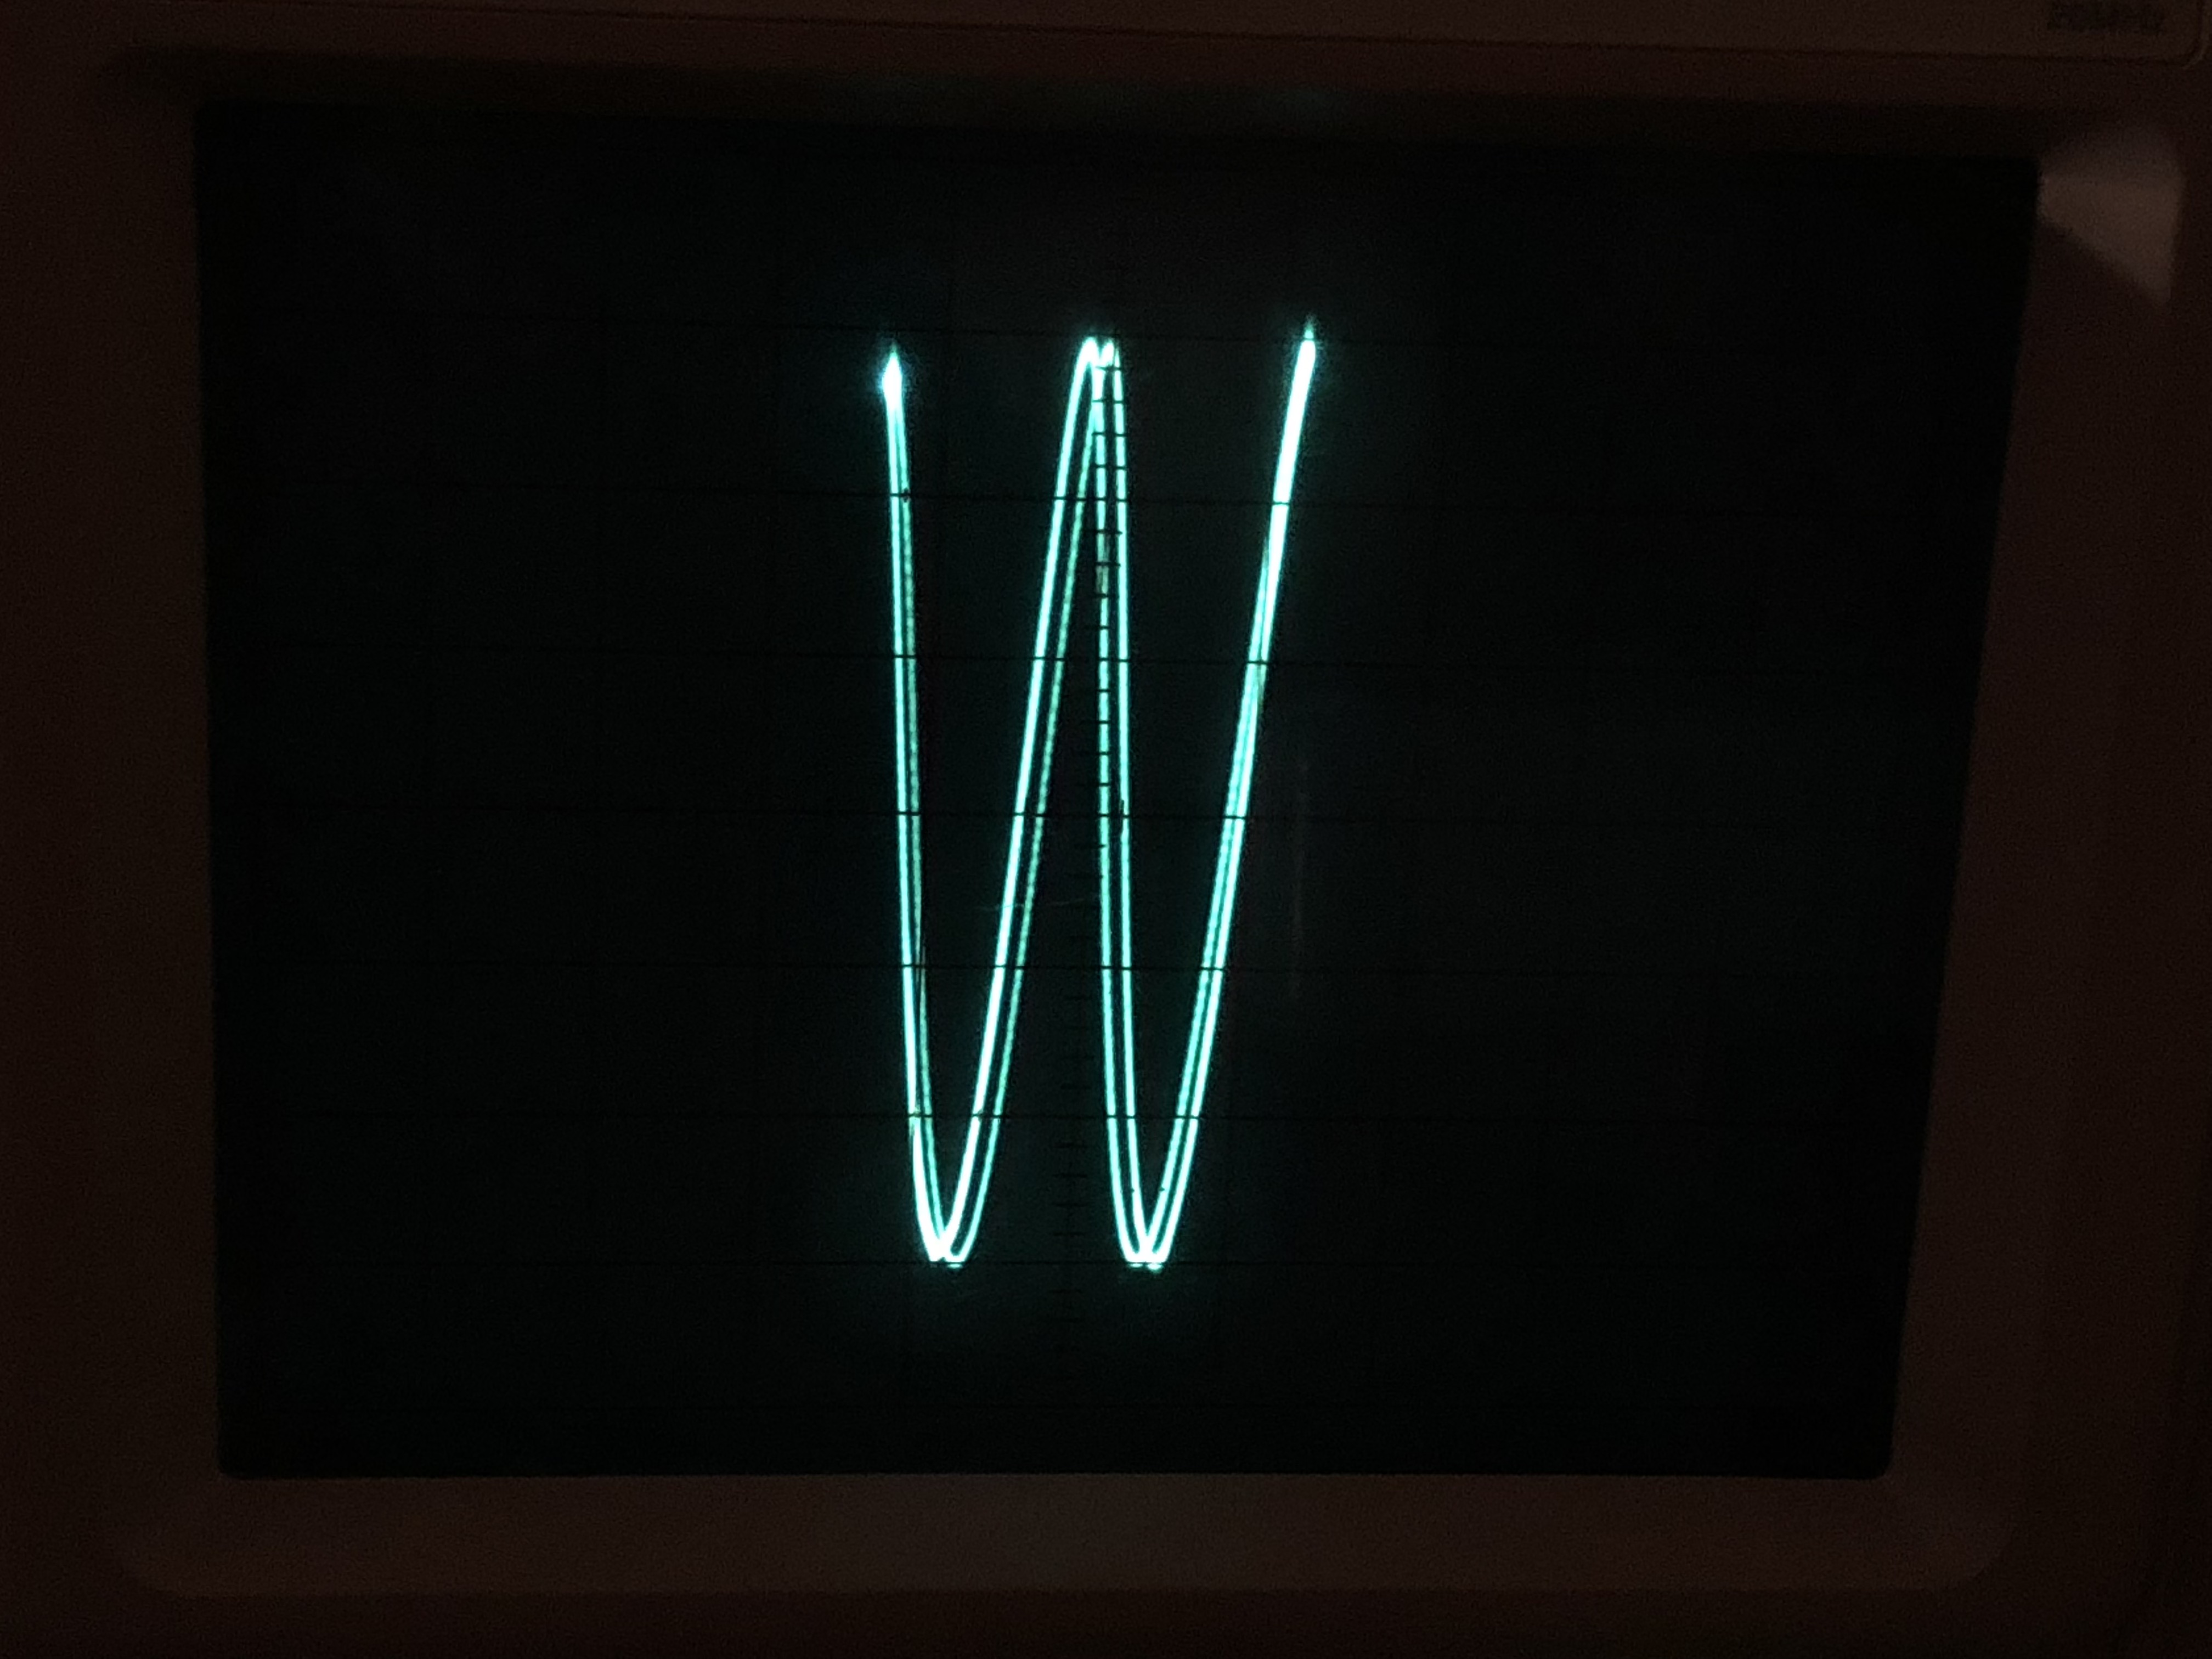
\includegraphics[width=0.7\linewidth]{lis2} \\ $U_\lambda$}
	\end{minipage}
	\hfill
	\begin{minipage}[h]{0.32\linewidth}
		\center{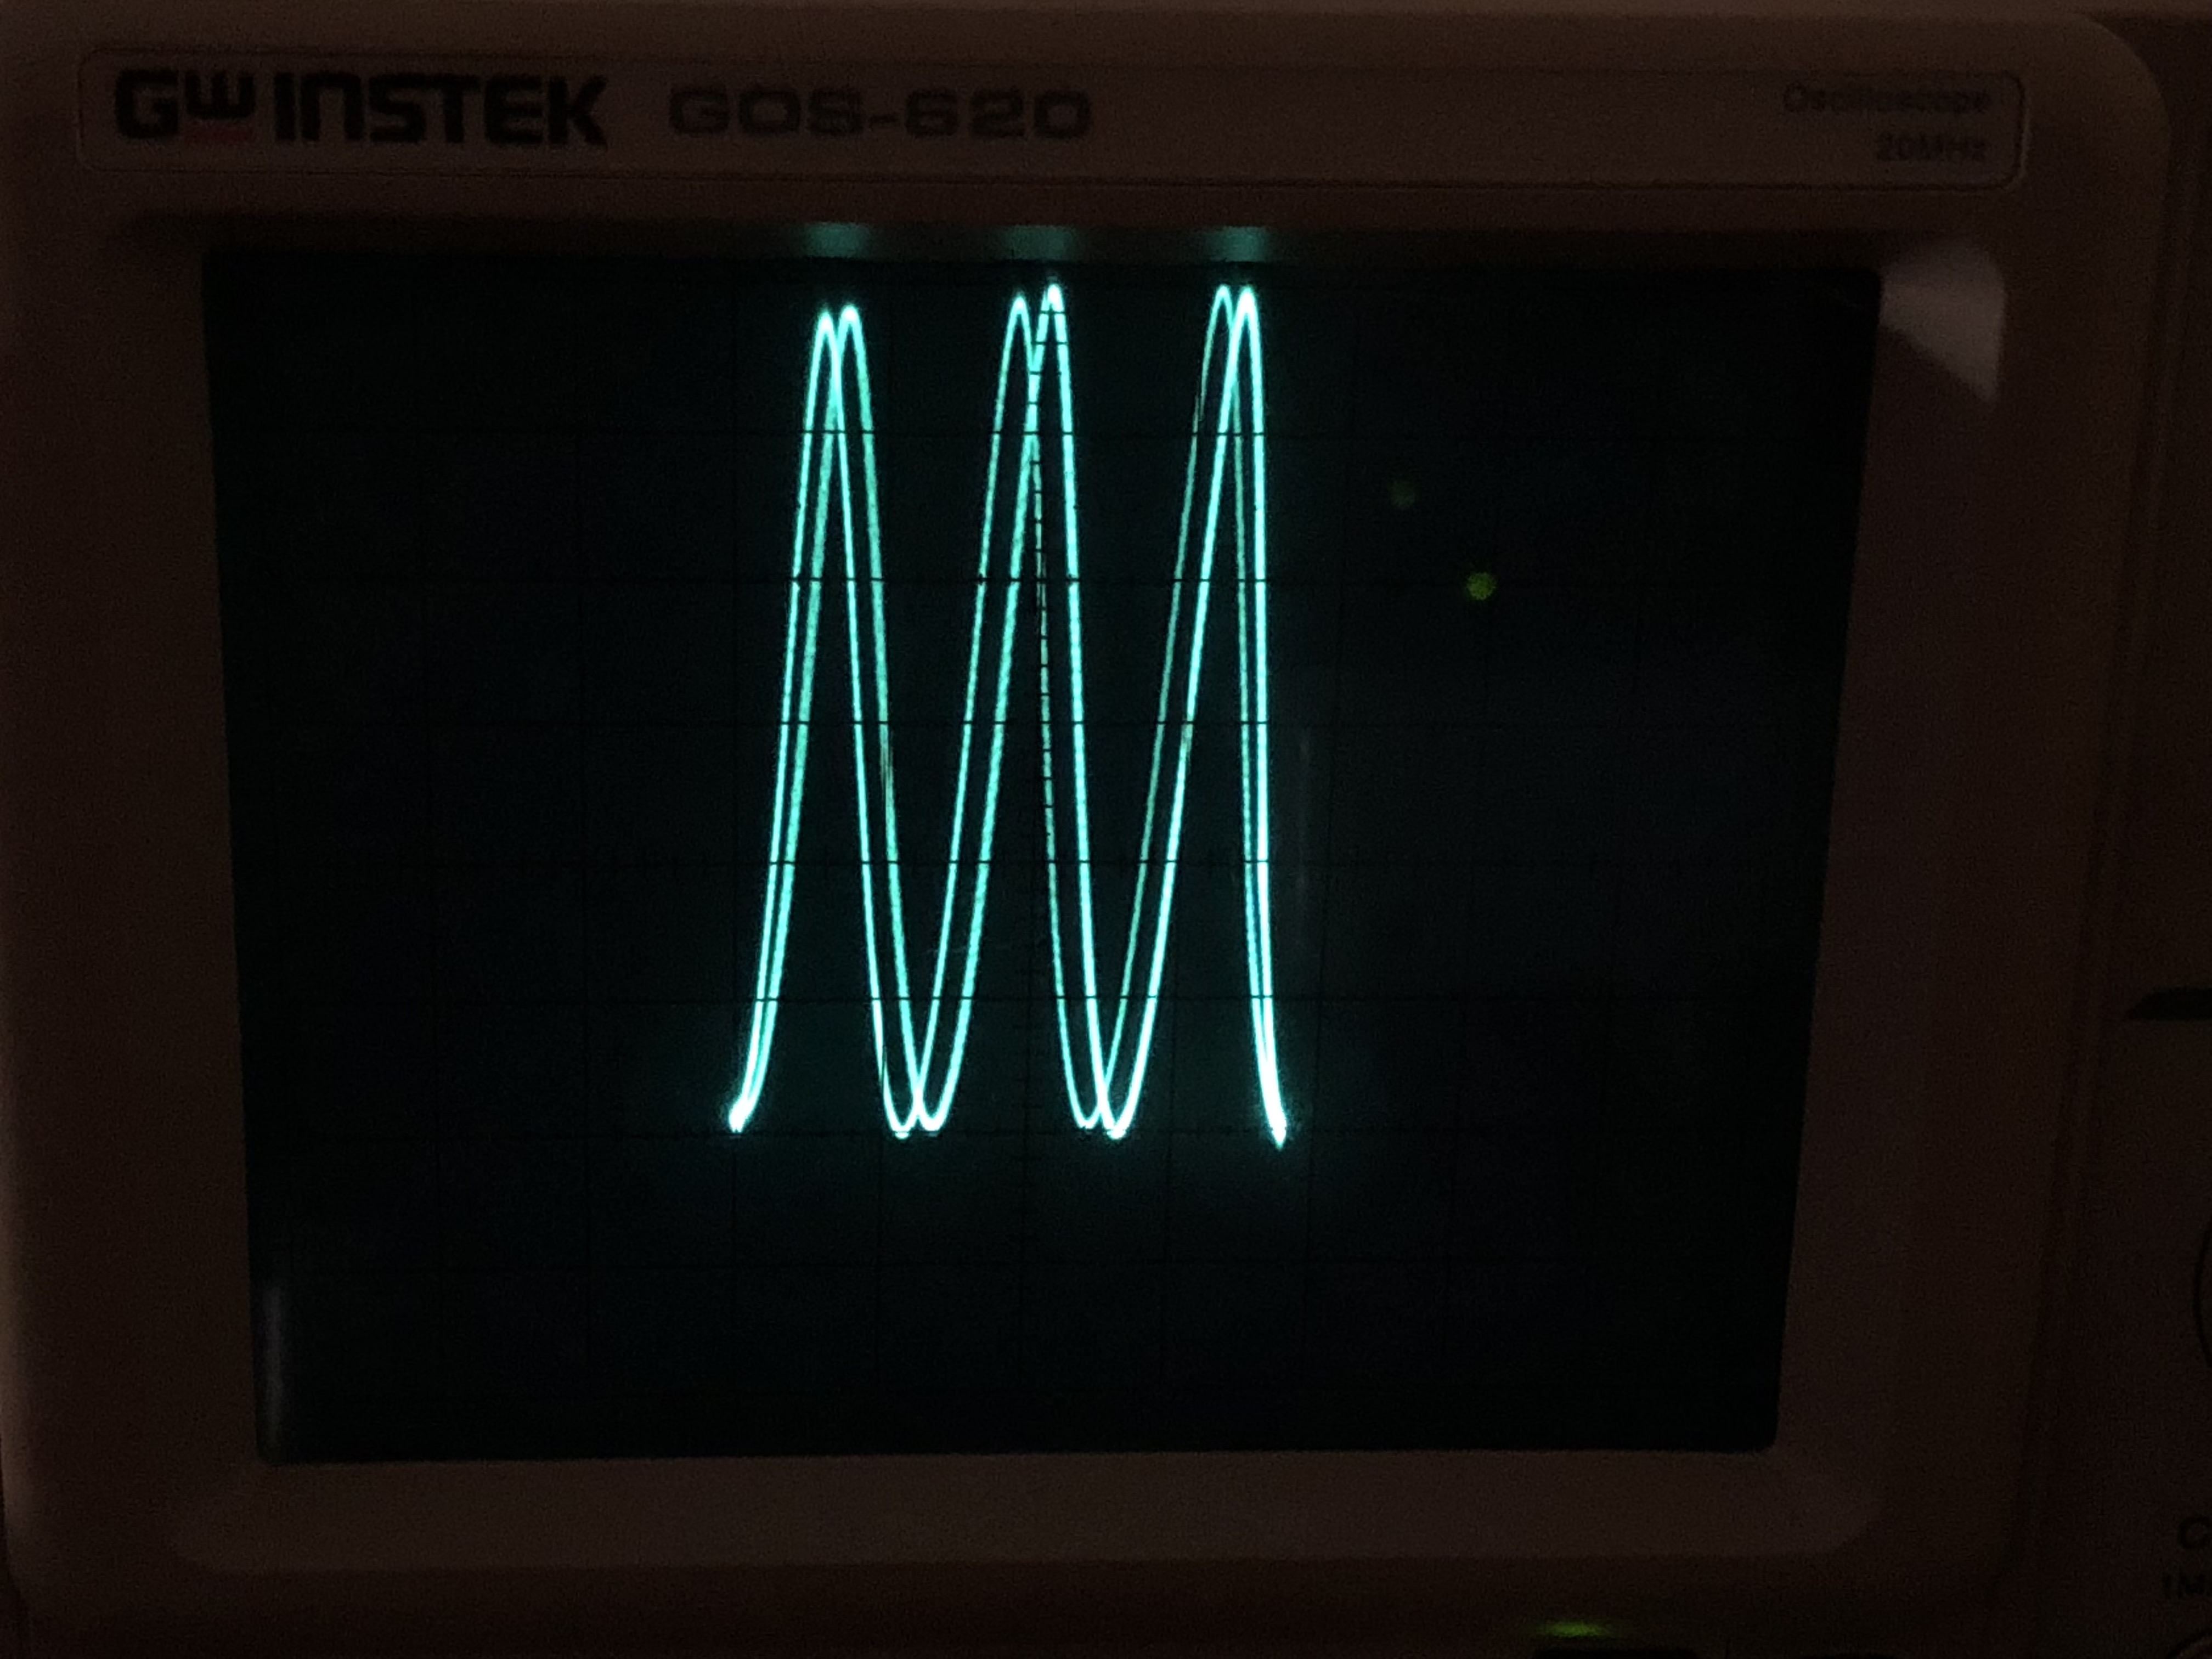
\includegraphics[width=0.7\linewidth]{lis3} \\ $U_{3\lambda/2} $}
	\end{minipage}
	\caption{Фигуры Лиссажу.}
	\label{ris:image1}
\end{figure}
\paragraph{Вывод.} Мы пронаблюдали эффект Поккельса и провели эксперимент, в следствии которого изменение показателя преломления света в кристалле под действием электрического поля, причем установили, что это изменение пропорционально напряженности электрического поля. Измерив радиусы интерференционных колец мы определили двулучепреломление ниобота лития, оно оказалось равным $ n_0 - n_e = 9.2 \pm 0.1 \cdot 10^{-2} $, т.е. с ошибкой не более чем 1\%. Подав на кристал постоянное напряжение получили свет, поляризованный по кругу и определили полуволновое напряжение $ U_{\lambda/2} = 465  $ В.
\end{document}
